\subsubsection{Effect of dataset dimensions}
\label{adverse}

Behaviors are compared on an easy setting ($n=100$, $p=20$) and a hard setting ($n=50$, $p=30$). Fig.~\ref{TPFN} displays FDR and density ratio measures for all methods on the different cases.  Detailed values of medians and standard-deviations are given in Tables \ref{medFDR} and \ref{meddens} in appendix. The behaviour of methods remains virtually the same across Erdös and Cluster structures. Scale-free structure appears to entail a greater difficulty for all methods with median FDR above $75\%$, except for EMtree which stays at $30\%$ in the hard setting. These poor performance are due to the inferred networks being too dense compared to the original Scale-free graphs. Another experiment with the Scale-free structure is detailed in Fig.~\ref{SF50}, where the number of species is fixed to $50$, and the number of samples is $100$ or $50$.  Under such setting the behavior of ecoCopula and MRFcov greatly improves with FDR at about $30\%$, where EMtree shows about $40\%$ in median (detailed values available in Table~\ref{perfSF50} in appendix).\\
The greater difficulty affects all methods. Density ratios either increase (MInt, SpiecEasi) or decrease (gCoda, ecoCopula, MRFcov). In the first case, FDRs tend to increase as well (e.g. $40\%$ increase for MInt in Erdös and Cluster structures), where a decrease in density ratio yields more empty results (e.g. in Table \ref{empty} $25\%$ of empty graphs for ecoCopula with  Erdös and Cluster structures, $15\%$ with Scale-free structures for $p$ fixed to $50$). EMtree seems to remain stable as for the density ratio, however it shows an increase in FDR measures of about $20\%$ for all structures.


Considering FDRs and density ratios combined, EMtree appears to be the method with the lower FDR which maintains a density ratio reasonably close to 1. As a consequence, the proposed methodology compares well to existing tools on problems with varying difficulties. EMtree is also comparable on running times. Table~\ref{timesTPFN} shows that for Erdös and Cluster it is the third quicker method in easy cases and the second in hard ones. Table \ref{timeSF} (in appendix) shows that on hard scale-free problems ($p=30$ and $p=50$ with $n=50$) EMtree is the quicker method, and third otherwise.

Interestingly, in easy cases when the network density is well estimated, methods yield FDR of $10\%-30\%$ in median. This reminds that network inference from abundance data is a difficult task, and that perfect inference of the network remains an out-of-reach goal. 
 
%\begin{figure}
%    \centering
%    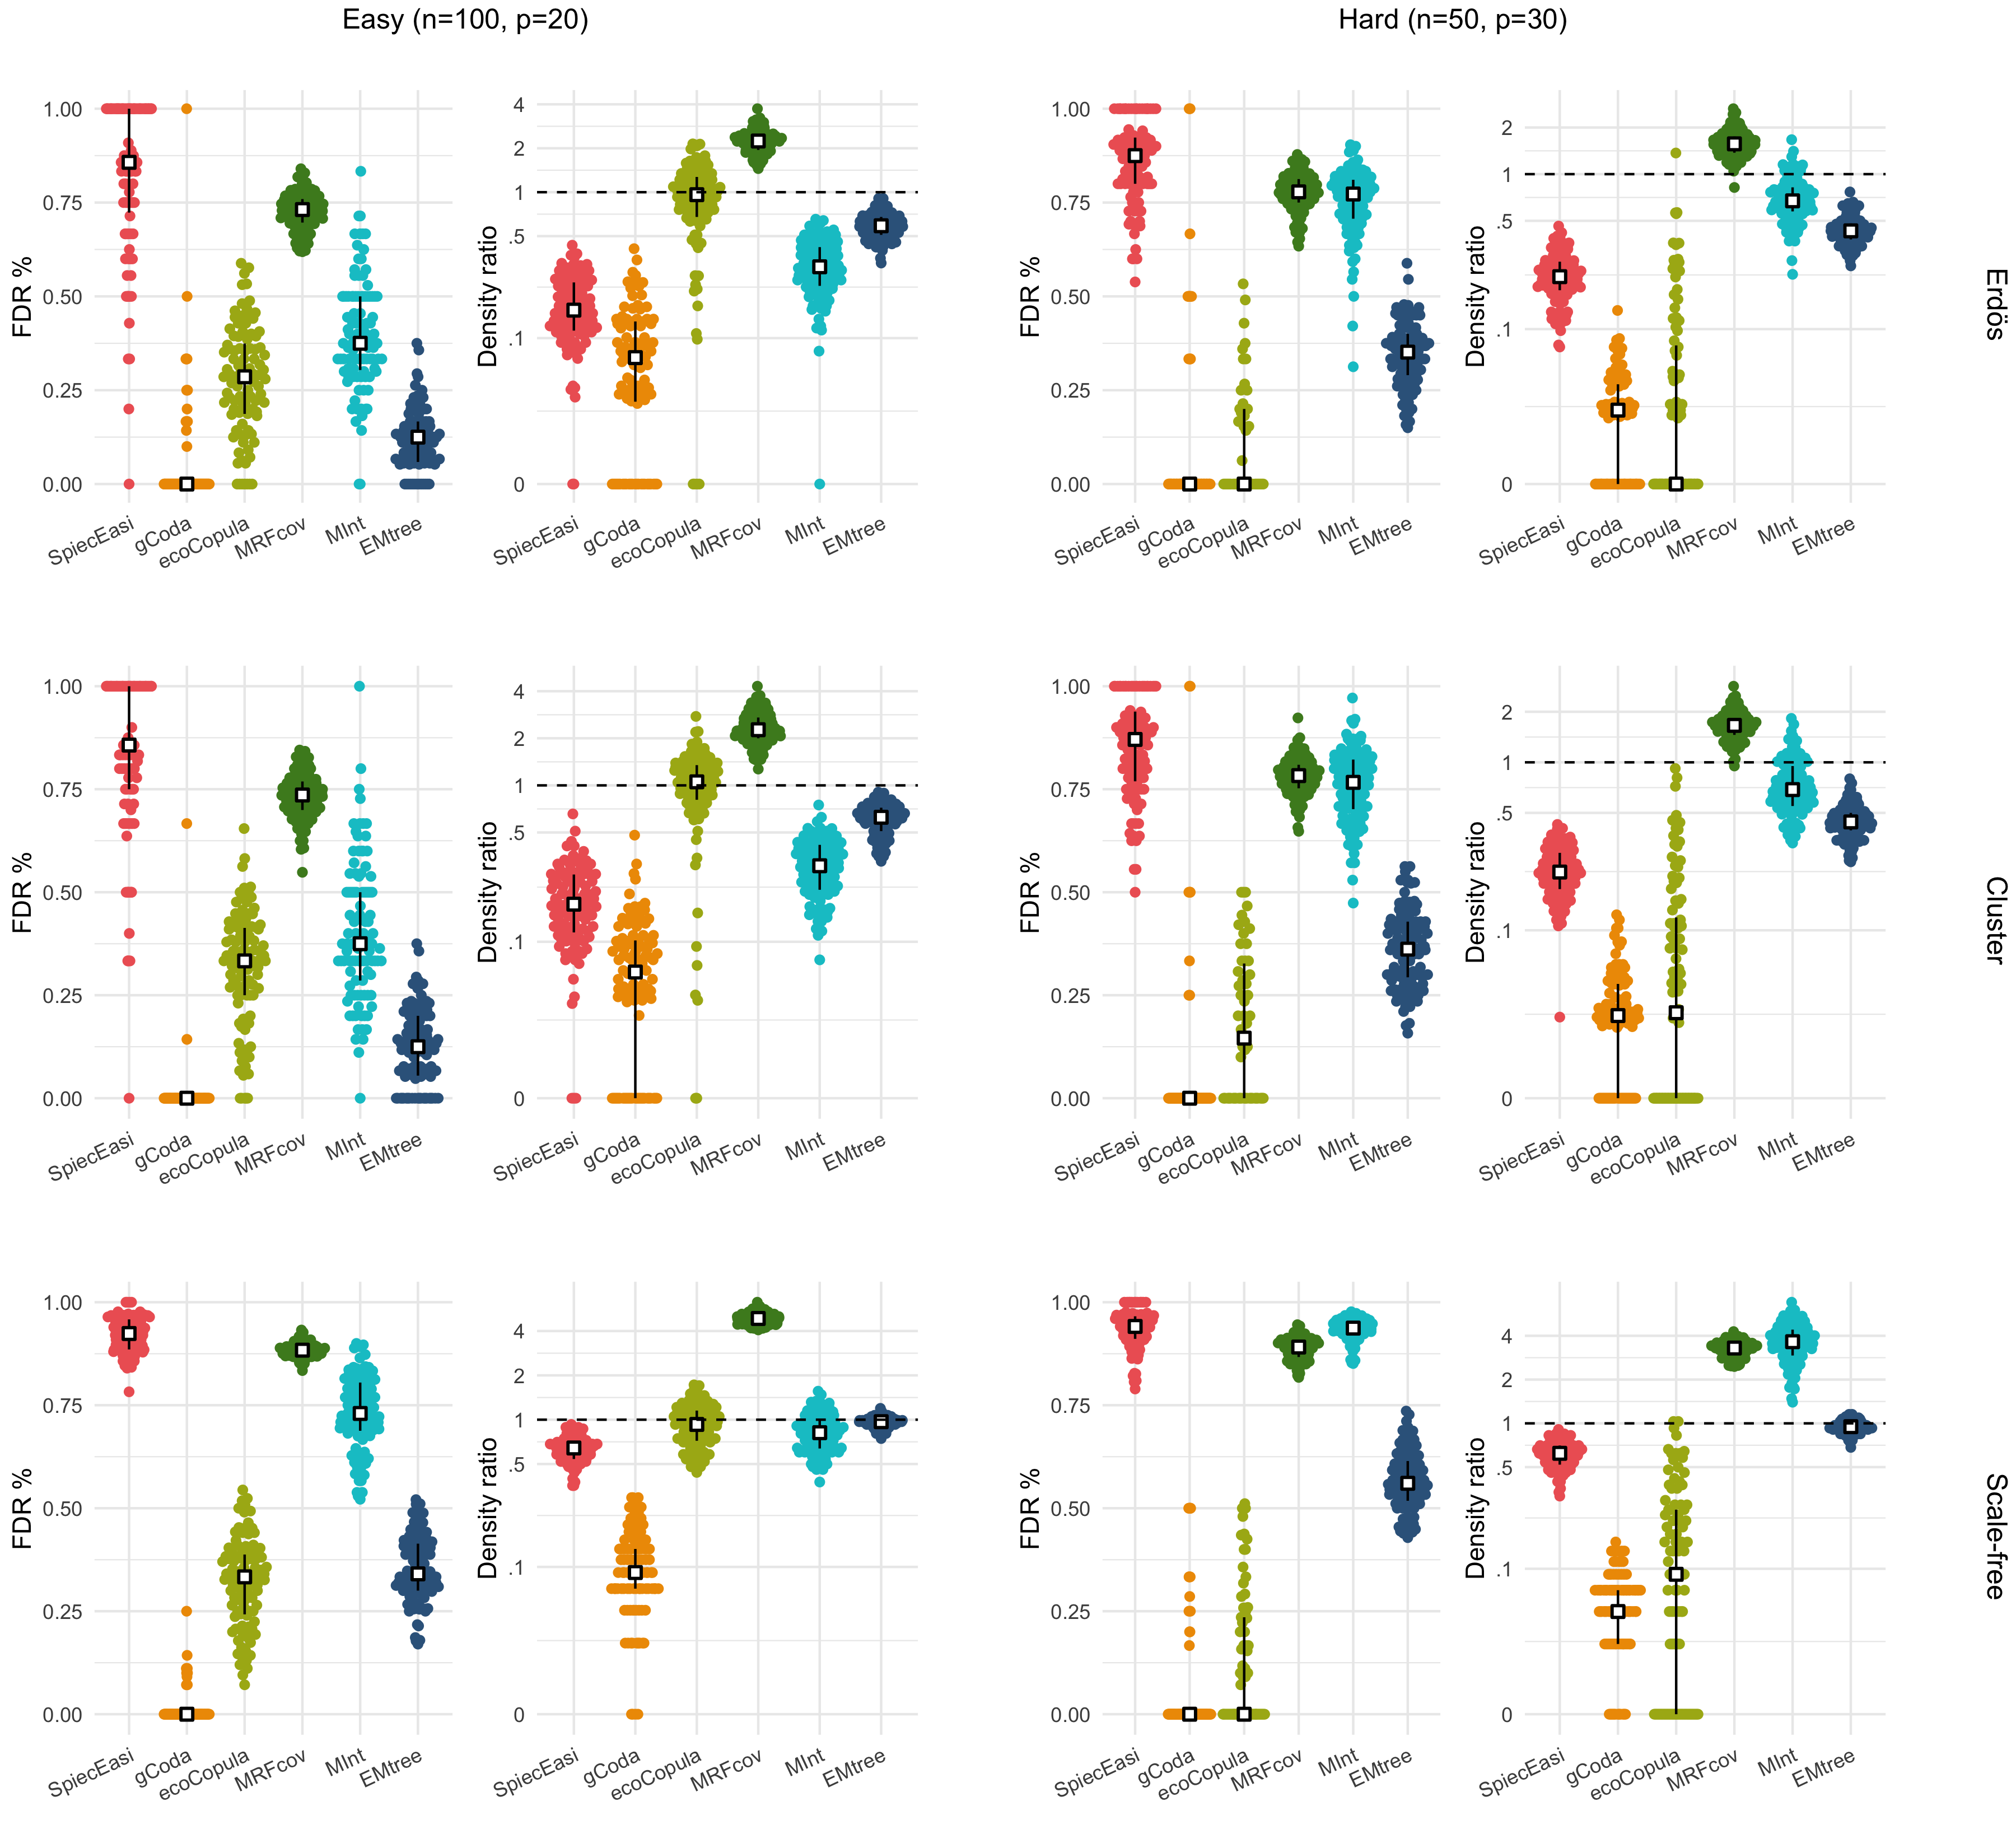
\includegraphics[width=\linewidth]{figs/panel_TPFN_signed.png}
%    \caption{FDR and density ratio measures for all methods at two different difficulty levels and 100 networks of each type. White squares and black plain lines represent medians and quartiles respectively. \small{\textit{ecoCopula selection method: AIC. Number of subsamples for SpiecEasi and EMtree: $S=20$. SpiecEasi and gCoda: $lambda.min.ratio=0.001$,  $nlambda=100$.}}}
%    \label{TPFN}
%\end{figure}

\begin{figure}
    \centering
    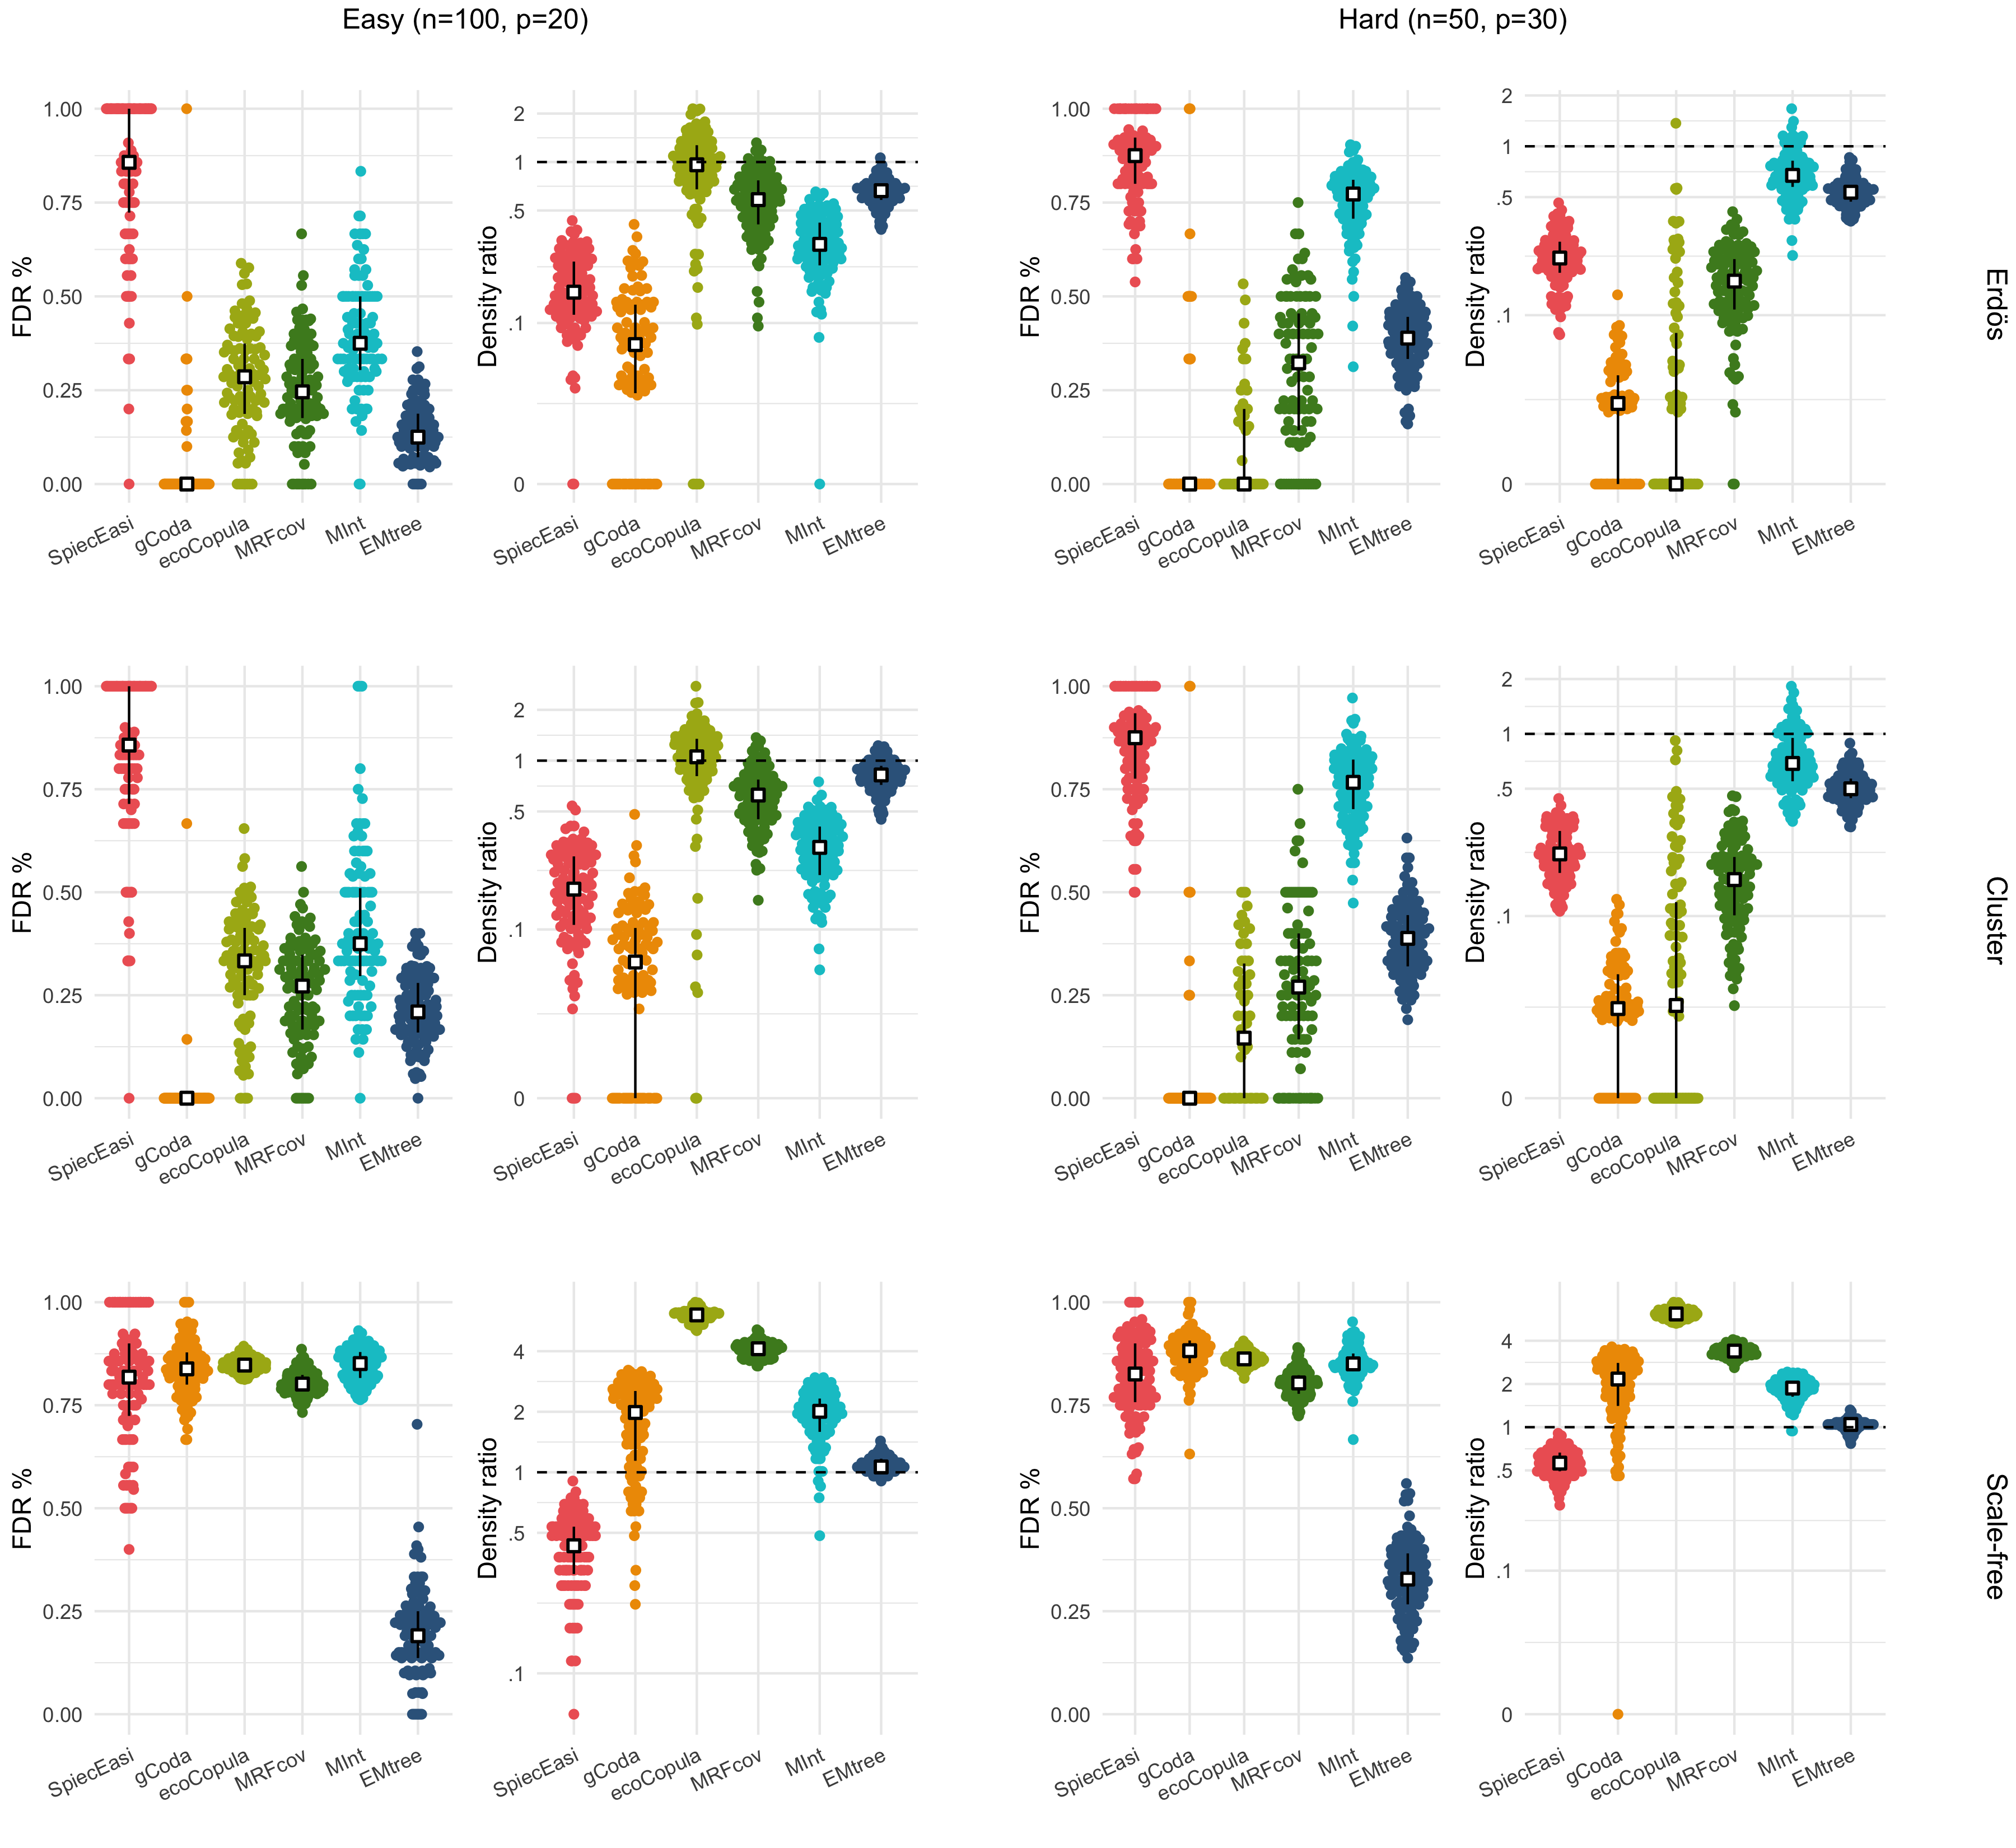
\includegraphics[width=\linewidth]{figs/correct_TPFN.png}
    \caption{FDR and density ratio measures for all methods at two different difficulty levels and 100 networks of each type. White squares and black plain lines represent medians and quartiles respectively. \small{\textit{ecoCopula selection method: AIC. Number of subsamples for SpiecEasi and EMtree: $S=20$. SpiecEasi and gCoda: $lambda.min.ratio=0.001$,  $nlambda=100$.}}}
    \label{TPFN}
\end{figure}
\begin{figure}
    \centering
    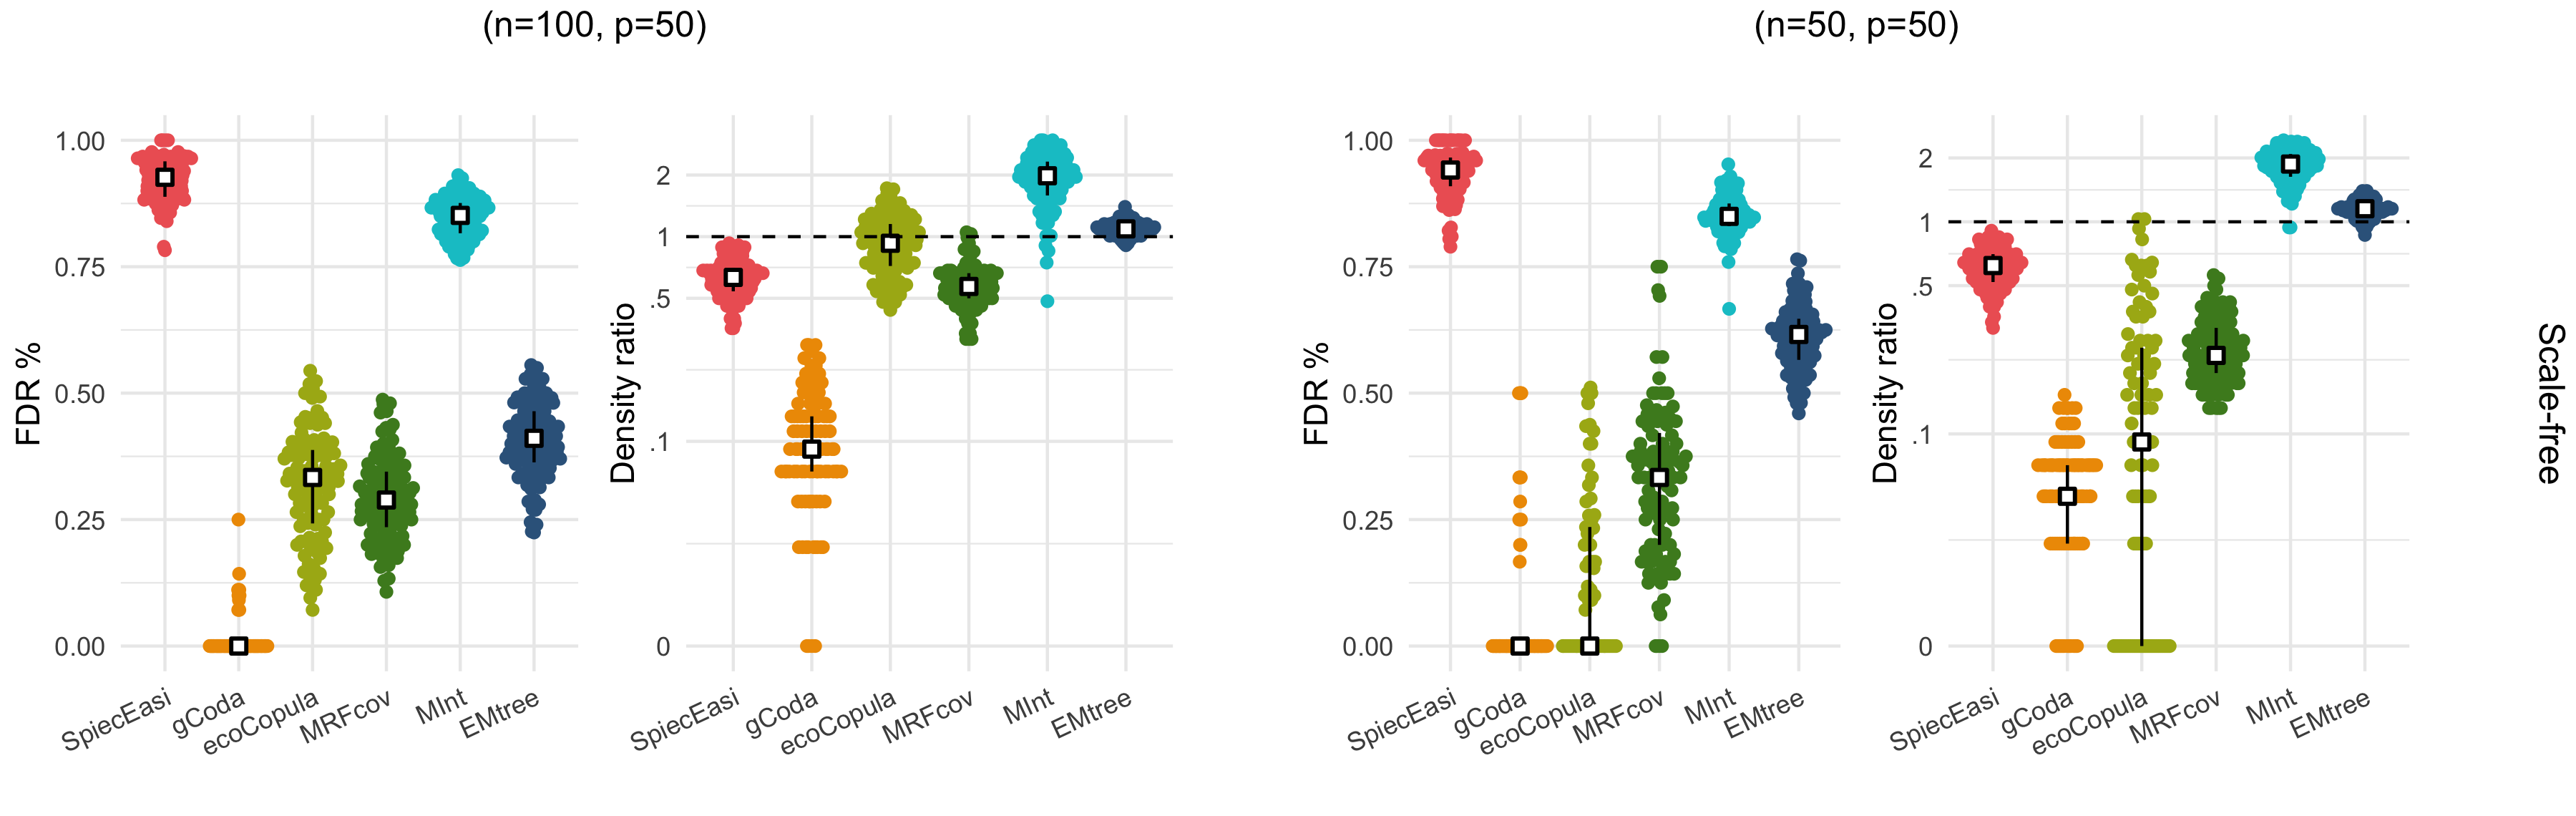
\includegraphics[width=\linewidth]{figs/BadSF_TPFN_title.png}
    \caption{FDR and density ratio measures for all methods on scale-free graphs with $p=50$. White squares and black plain lines represent medians and quartiles respectively. \small{\textit{ecoCopula selection method: AIC. Number of subsamples for SpiecEasi and EMtree: $S=20$. SpiecEasi and gCoda: $lambda.min.ratio=0.001$,  $nlambda=100$.}}}
    \label{SF50}
\end{figure}

\begin{table}
\centering
 
\begin{tabular}{l|rrrrrr}
 & \multicolumn{1}{c}{SpiecEasi} & \multicolumn{1}{c}{gCoda} & \multicolumn{1}{c}{ecoCopula} & \multicolumn{1}{c}{MRFcov} & \multicolumn{1}{c}{MInt} & \multicolumn{1}{c}{EMtree} \\ 
  \hline
Easy &  19.99(4.19) & 0.1(0.05) & 4.2(0.24) & 5.76(0.35) & 54(26.9) & 4.44(0.64) \\ 
  Hard &  24.29(5.07) & 0.5(0.24) & 8.19(0.16) & 5.52(2.98) & 33.87(18.37) & 3.29(0.32)  \\ 
   \hline
\end{tabular}
\caption{Median and standard-deviation running-time values (in seconds) for Cluster and Erdös structures, including resampling with $S=20$ for SpiecEasi and EMtree.}
\label{timesTPFN}
\end{table}




%%%%%%%%%%%%%%%%%%%%%%%%%%%%%%%%%%%%
%%%%%%%%%%%%%%%%%%%%%%%%%%%%%%%%%%%%

\subsubsection{Effect of network structure}

As expected for a fixed $p$, the higher the number of observations $n$, the better the performance for all methods and structures. Interestingly, the same happens when $p$ increases for a fixed $n=100$ (except for SpiecEasi).
EMtree performs well on Scale-free structures (Fig.~\ref{SFAUC}) which was also expected; the other methods performance worsen compared to other structures. When lowering $n$ to 30, EMtree performance deteriorates along with $p$, yet remaining above $70\%$ in median in the extreme case where $p=n$ (Fig.~\ref{SFAUC}, right). The structure being Erdös or Cluster, each method is affected in the same way by an increase of $n$ or $p$ (Fig.~\ref{panelErdClust}). Besides, increasing the difference between the two structures by tuning up the \textit{ratio} parameter has no effect. Overall EMtree performs better than gCoda and SpiecEasi on all the studied configurations. Running times are summarized in Table~\ref{timeNP}. EMtree is about 10 times slower than gCoda (4 for small $n$), and 4 times faster than SpiecEasi. The high standard deviation for small $n$ seems to be due to gCoda struggling with Scale-free structures.
  
\begin{figure}[H]
    \centering
    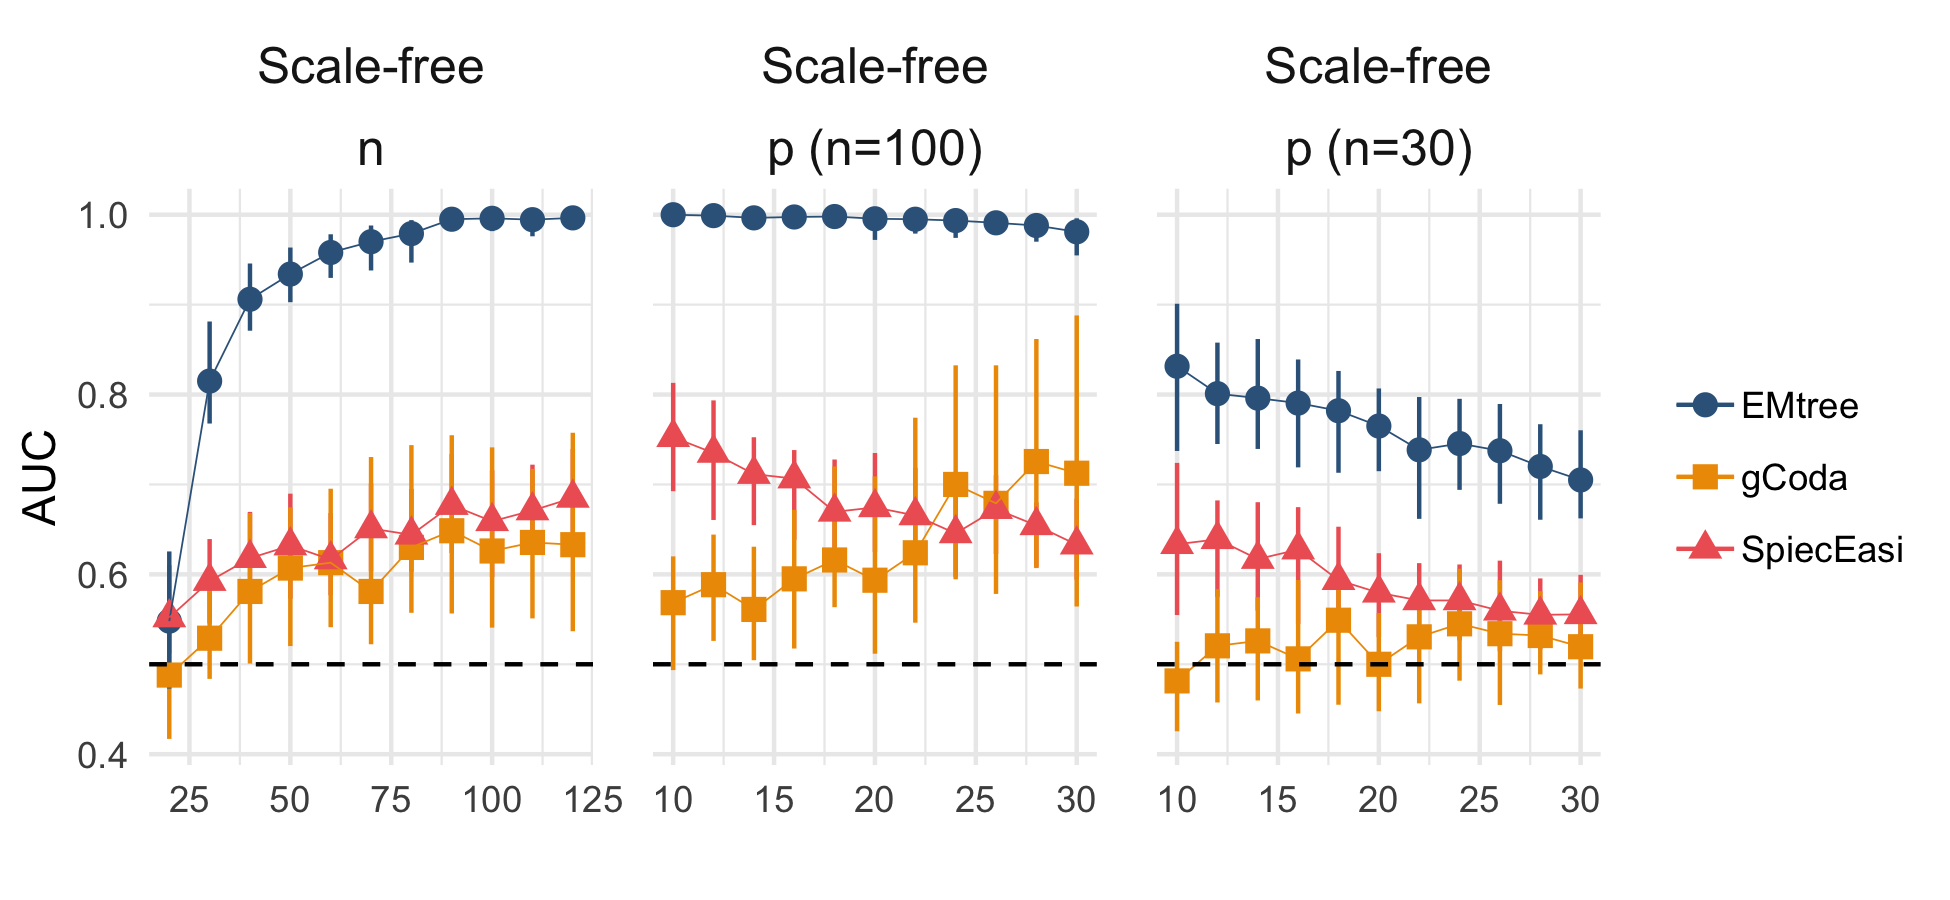
\includegraphics[width=0.7\linewidth]{figs/panel_SF.png}
    \caption{Effect of Scale-free structure on AUC medians and inter-quartile intervals for parameters $n$ and $p$.}
      \label{SFAUC}
\end{figure}


\begin{table}[H]
\centering
\begin{tabular}{l|rr|rr}
 & \multicolumn{1}{c}{$n < 50$} & \multicolumn{1}{c}{$n\geq 50$}  & \multicolumn{1}{c}{$p < 20$} & \multicolumn{1}{c}{$p\geq 20$} \\  
 \hline
  EMtree    &   0.44 (0.14)	 &   0.60 (0.17) &   0.41 (0.13) &   0.76 (0.21)   \\ 
  gCoda     &   0.11 (26.8)	 &   0.05 (0.05) &   0.05 (0.04) &   0.09 (0.54)   \\ 
  SpiecEasi &   2.09 (0.26)	 &   2.37 (0.28) &   2.42 (0.27) &   2.42 (0.26)   \\ 
   \hline
\end{tabular}
\caption{Median and standard-deviation of running times for each method in seconds, for $n$ and $p$ parameters.}
\label{timeNP}
\end{table}

%%%%%%%%%%%%%%%%%%%%%%%%%%%%%%%%%%%%
%%%%%%%%%%%%%%%%%%%%%%%%%%%%%%%%%%%%

\subsubsection{Effect of network density}
The comparison of top and bottom panels of Fig.~\ref{panelErdClust} shows that network inference gets harder as the network gets denser, whatever the method and the structure of the true graph. Running times are not affected (Table \ref{timeDenser}).
Fig.~\ref{varyDens} shows that EMtree performance does not deteriorate faster than that of other methods, demonstrating that the tree hypothesis is not a limitation.


 \begin{figure}[H]
  \centering
   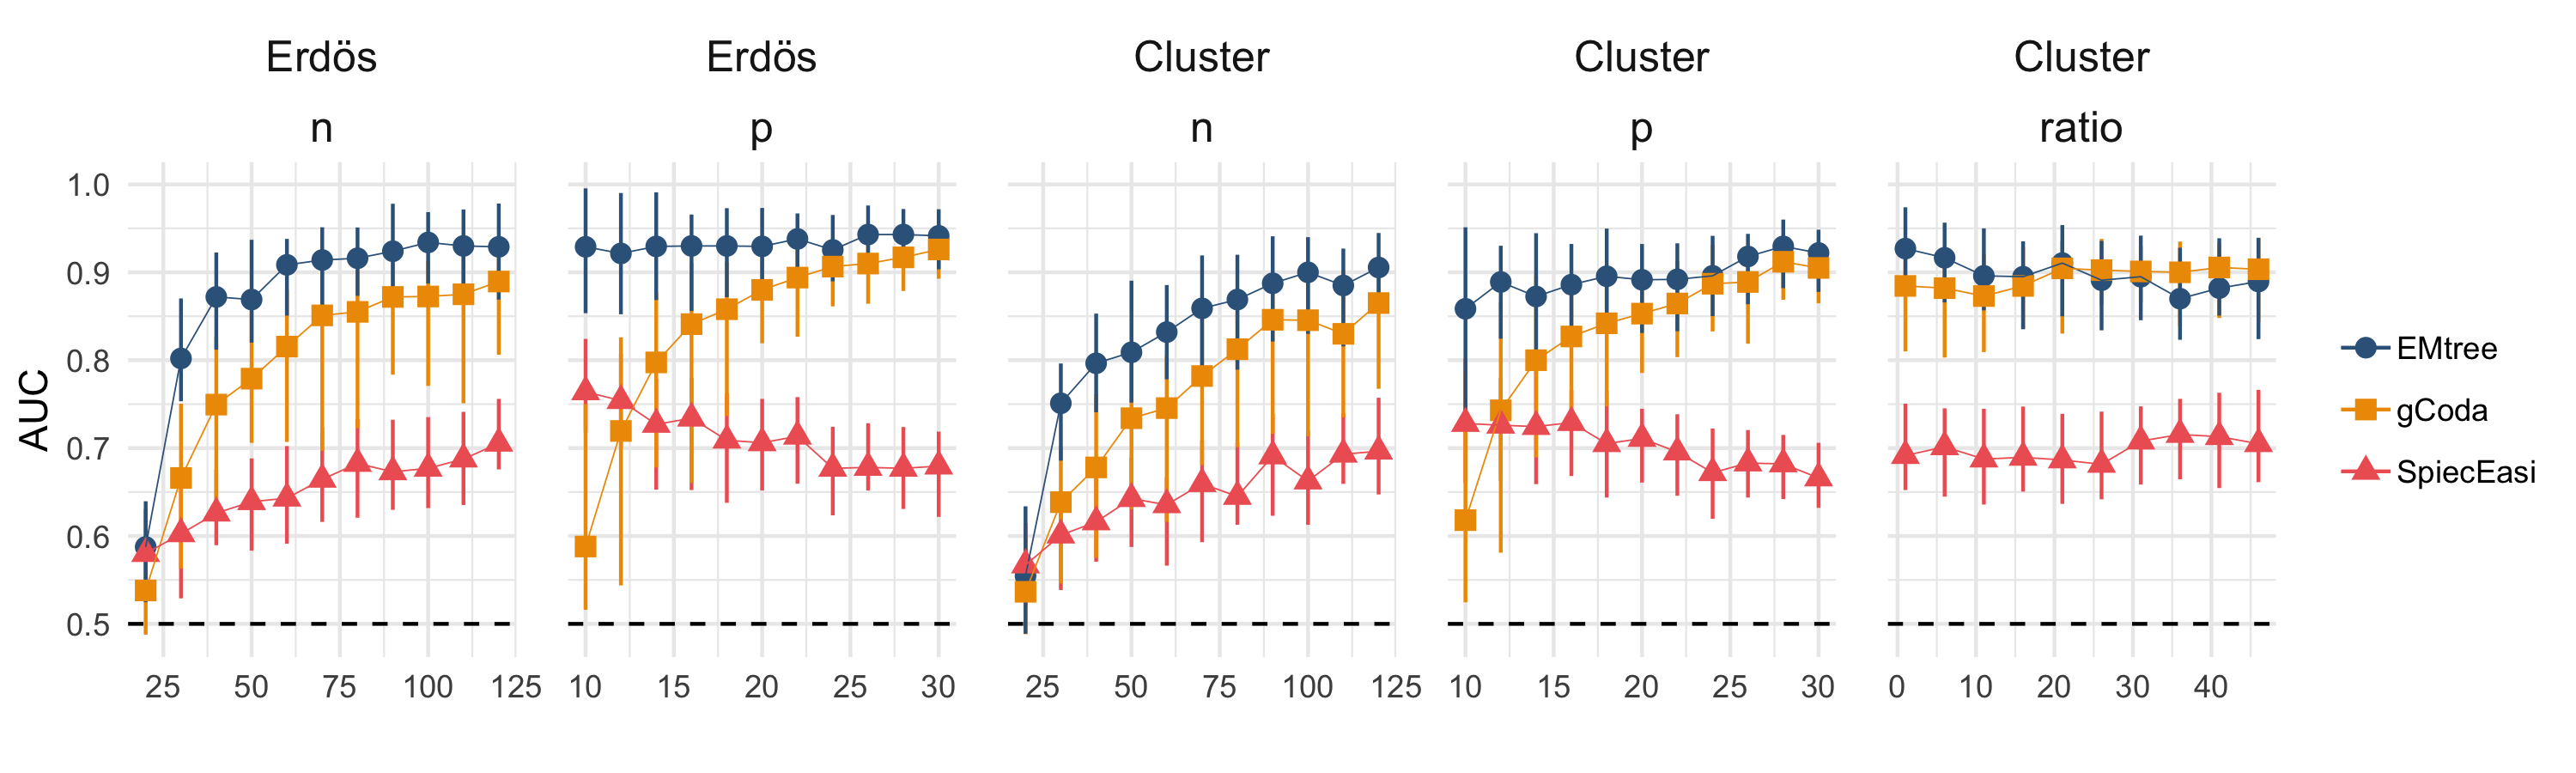
\includegraphics[width=\linewidth]{figs/panel_npFav.png}
  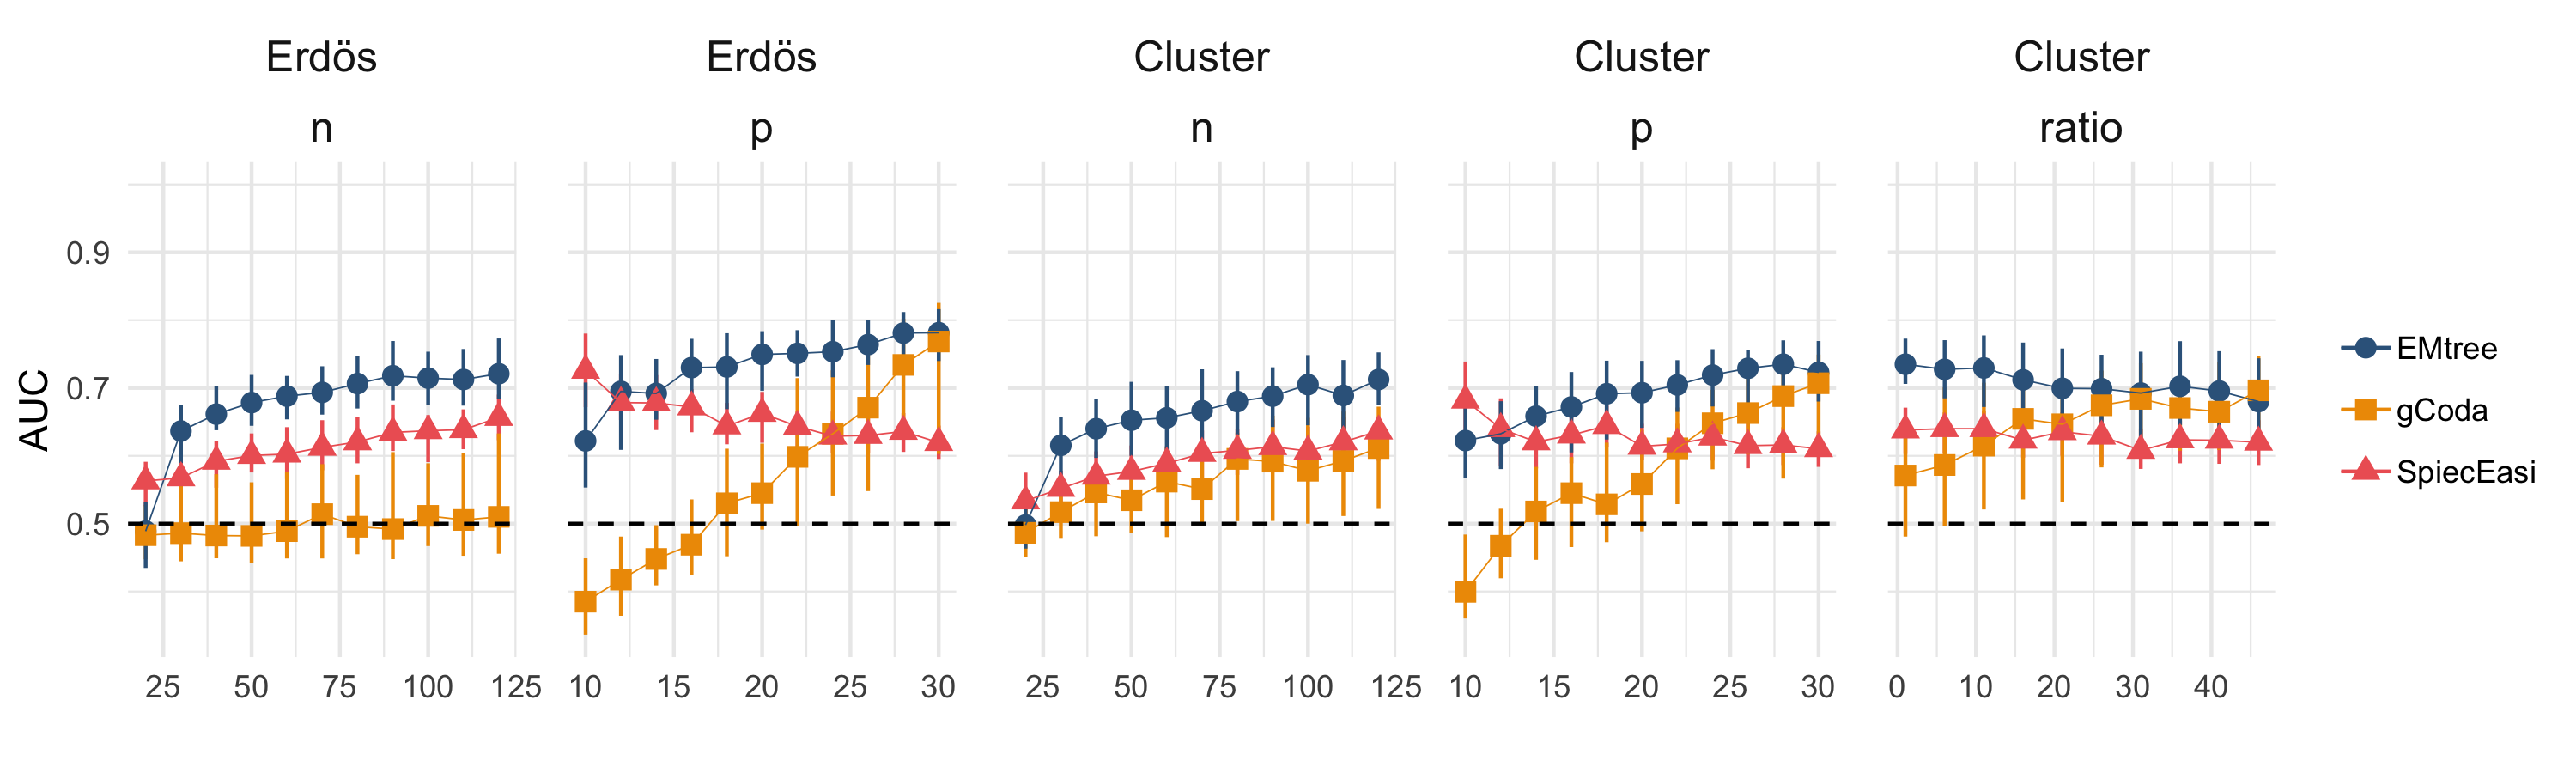
\includegraphics[width=\linewidth]{figs/panel_dense.png}
  \caption{Effect of Erdös and Cluster structures on AUC medians and inter-quartile intervals for parameters $n$, $p$ and $ratio$. \textit{Top}: densities set to $2/p$, \textit{bottom}: densities set to $5/p$.}
  \label{panelErdClust}
\end{figure}

\begin{figure}[H]
 \centering
  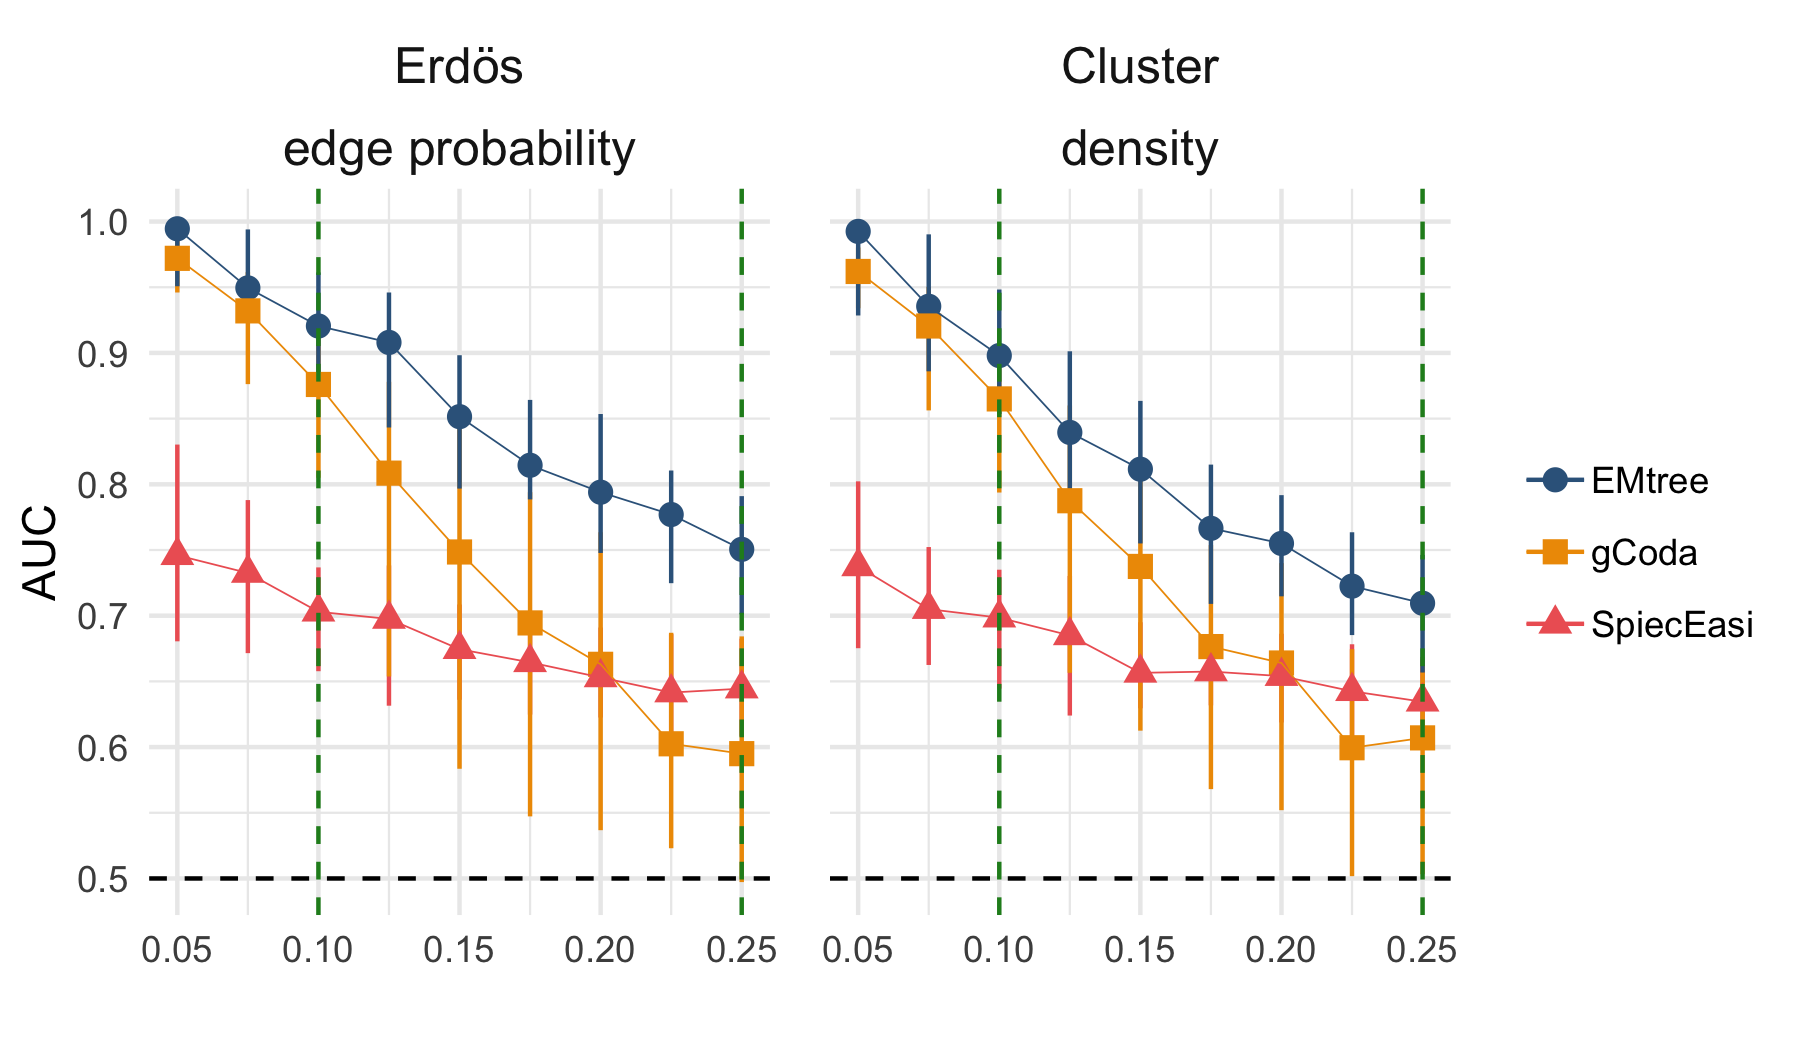
\includegraphics[width=0.6\linewidth]{figs/panel_dens_seuils.png}
  \caption{AUC median and inter-quartile intervals for parameters controlling the number of edges in Erdös (\textit{edge probability}) and in Cluster (\textit{density}) structures, $p=20$, $n=100$. The two vertical dotted lines are the $3/p$ and $5/p$ values.}
  \label{varyDens}
\end{figure}
 
